\documentclass[11pt,letterpaper]{article}

\usepackage[margin=1in]{geometry}
\usepackage{setspace}
\onehalfspacing

\usepackage{microtype}
\usepackage{booktabs}
\usepackage{longtable}
\usepackage{array}
\usepackage{tabularx}
\usepackage{xcolor}
\usepackage{amsmath,amssymb}
\usepackage{tikz}
\usetikzlibrary{shapes.geometric, arrows.meta, positioning, fit, backgrounds}
\usepackage[hyphens]{url}
\usepackage[colorlinks=true,linkcolor=blue,citecolor=blue,urlcolor=blue]{hyperref}
\usepackage{cleveref}
\usepackage[numbers,sort&compress]{natbib}

\definecolor{rustcolor}{HTML}{DEA584}
\definecolor{cppcolor}{HTML}{659AD2}
\definecolor{pythoncolor}{HTML}{3776AB}

\title{
    \vspace{-1cm}
    \textbf{Update 13: Lock-Free C++/Rust RDMA Middleware} \\[0.5em]
    \large Replacing Python Middleware with Cache-Line-Aware, Lock-Free Transport
}

\author{
    Nathan Gopee \\
    \textit{MS Computer Science Candidate} \\
    SUNY New Paltz \\
    \texttt{gopeen1@newpaltz.edu}
}

\date{February 2026}

\begin{document}

\maketitle

\begin{abstract}
\noindent
This update presents a migration plan from the current Python-based RDMA middleware (pyverbs, WFA classifier, dual-path router) to a low-level C++/Rust implementation using lock-free data structures, cache-line-aligned memory layouts, and direct libibverbs/librdmacm bindings. The plan leverages existing lock-free patterns from the Neumann tensor runtime (HLC, Raft atomics, entity index) and integrates with UCX, OpenMPI, and vLLM at the systems level. An SPSC (Single-Producer/Single-Consumer) ring buffer forms the core data structure for zero-copy tensor transport between RDMA completion threads and application threads.
\end{abstract}

\section{Motivation: Why Leave Python}

The current middleware prototype implements five Python modules:

\begin{table}[htbp]
\centering
\caption{Current Python middleware components}
\label{tab:python-middleware}
\begin{tabular}{@{}llp{7cm}@{}}
\toprule
\textbf{Module} & \textbf{Lines} & \textbf{Purpose} \\
\midrule
\texttt{wfa\_classifier.py} & 30 & WFA tensor hot/warm/cold classification \\
\texttt{rdma\_buffer\_pool.py} & 15 & NUMA-aware RDMA buffer pool (pyverbs MR) \\
\texttt{dual\_path\_rdma.py} & 25 & Hot/cold QP routing with batching \\
\texttt{transports.py} & 90 & Transport abstraction (TCP/RoCE/TTPoe) \\
\texttt{vllm\_connector.py} & 30 & Adaptive RDMA connector for vLLM KV cache \\
\bottomrule
\end{tabular}
\end{table}

These prototypes validated the architecture but cannot serve as production middleware for three reasons:

\begin{enumerate}
    \item \textbf{GIL contention.} Python's Global Interpreter Lock serializes all RDMA completion handling. The pyverbs \texttt{poll\_completion()} loop (1~ms sleep interval) adds $>$1~ms of latency per operation---two orders of magnitude above the hardware floor.

    \item \textbf{No cache-line control.} Python allocates objects on the heap with arbitrary alignment. False sharing between producer and consumer indices in ring buffers cannot be prevented, and NUMA-aware placement requires \texttt{ctypes} hacks that defeat the purpose of using Python.

    \item \textbf{Memory registration overhead.} Every pyverbs \texttt{MR(pd, size, flags)} call triggers a kernel \texttt{ibv\_reg\_mr} syscall. In C/C++/Rust, memory can be pre-registered once and suballocated via a slab allocator with zero additional syscalls.
\end{enumerate}

\section{Existing Lock-Free Infrastructure}

The Neumann tensor runtime (submodule, 400K+ lines of Rust) already implements several lock-free patterns that can be extended for RDMA transport:

\subsection{Hybrid Logical Clock (\texttt{hlc.rs})}

The HLC implementation (583 lines) generates causally ordered timestamps using a CAS (compare-and-swap) retry loop over two \texttt{AtomicU64} fields: \texttt{last\_wall\_ms} and \texttt{logical}. When the wall clock advances, the thread atomically swaps the stored wall time via \texttt{compare\_exchange} and resets the logical counter. On CAS failure (another thread won the race), it retries. When the wall clock has not advanced, it monotonically increments the logical counter via \texttt{fetch\_add}. Both paths use \texttt{SeqCst} ordering. This CAS-retry-with-monotonic-progress pattern directly maps to RDMA completion ordering, where multiple completion threads must agree on a global sequence number for work requests.

\subsection{Raft Consensus Atomics (\texttt{raft.rs})}

The Raft implementation uses \texttt{AtomicU64} with \texttt{Ordering::Relaxed} for statistics (heartbeat counters, fast-path metrics) and \texttt{Ordering::SeqCst} for critical state (finalized height, compaction epoch). This two-tier ordering strategy---relaxed for hot counters, sequentially consistent for correctness boundaries---is the same approach needed for RDMA work request tracking.

\subsection{Loom Concurrency Testing (\texttt{loom\_raft.rs})}

Neumann uses the \texttt{loom} crate for deterministic concurrency testing under all possible thread interleavings. The RDMA SPSC ring buffer will use the same approach to verify correctness.

\subsection{Entity Index with Append-Only Vocabulary (\texttt{entity\_index.rs})}

The \texttt{EntityIndex} uses \texttt{AtomicU64} for the next-ID counter and \texttt{parking\_lot::RwLock} for the hash index---demonstrating the pattern of combining lock-free hot paths with locked cold paths, which maps directly to the RDMA dual-path architecture (lock-free hot QP, locked cold batch).

\section{Architecture: Lock-Free RDMA Transport}

\begin{figure}[htbp]
\centering
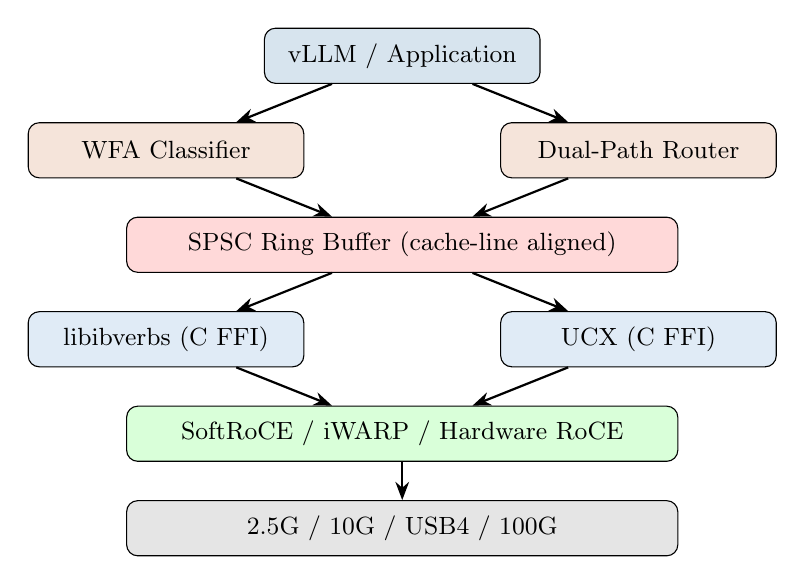
\begin{tikzpicture}[
    node distance=0.6cm,
    box/.style={rectangle, draw, rounded corners, minimum width=3.5cm, minimum height=0.7cm, align=center, font=\small},
    arrow/.style={->, thick, >=Stealth}
]
    % Application layer
    \node[box, fill=pythoncolor!20] (vllm) at (0,6) {vLLM / Application};

    % Rust middleware
    \node[box, fill=rustcolor!30] (wfa) at (-3,4.8) {WFA Classifier};
    \node[box, fill=rustcolor!30] (router) at (3,4.8) {Dual-Path Router};

    % SPSC ring buffers
    \node[box, fill=red!15, minimum width=7cm] (spsc) at (0,3.6) {SPSC Ring Buffer (cache-line aligned)};

    % C++ RDMA layer
    \node[box, fill=cppcolor!20] (verbs) at (-3,2.4) {libibverbs (C FFI)};
    \node[box, fill=cppcolor!20] (ucx) at (3,2.4) {UCX (C FFI)};

    % Transport
    \node[box, fill=green!15, minimum width=7cm] (transport) at (0,1.2) {SoftRoCE / iWARP / Hardware RoCE};

    % Network
    \node[box, fill=gray!20, minimum width=7cm] (net) at (0,0) {2.5G / 10G / USB4 / 100G};

    \draw[arrow] (vllm) -- (wfa);
    \draw[arrow] (vllm) -- (router);
    \draw[arrow] (wfa) -- (spsc);
    \draw[arrow] (router) -- (spsc);
    \draw[arrow] (spsc) -- (verbs);
    \draw[arrow] (spsc) -- (ucx);
    \draw[arrow] (verbs) -- (transport);
    \draw[arrow] (ucx) -- (transport);
    \draw[arrow] (transport) -- (net);
\end{tikzpicture}
\caption{Lock-free RDMA middleware architecture. Rust components (orange) communicate with C FFI layers (blue) through cache-line-aligned SPSC ring buffers (red).}
\label{fig:lockfree-arch}
\end{figure}

\section{Core Component: SPSC Ring Buffer}

The SPSC (Single-Producer/Single-Consumer) ring buffer is the central data structure. Informed by the LMAX Disruptor pattern~\cite{disruptor} and the USENIX ATC 2022 BBQ paper~\cite{bbq-usenix}, the design eliminates all locks on the hot path.

\subsection{Cache-Line Layout}

False sharing between producer and consumer indices is the primary performance killer in na\"ive ring buffer implementations~\cite{drepper2007memory}. The solution is to place each index on its own 64-byte cache line using \texttt{\#[repr(C, align(64))]} structs. The \texttt{ProducerState} contains the atomic \texttt{head} index (written only by the producer) and a thread-local \texttt{cached\_tail} copy of the consumer's position. The \texttt{ConsumerState} mirrors this with \texttt{tail} and \texttt{cached\_head}. Both structs are explicitly padded to 64 bytes so that they never share a cache line. The ring buffer itself holds a power-of-two-sized slot array and a bitmask (\texttt{capacity $-$ 1}) for index-to-slot conversion without modulo division.

\subsection{Producer/Consumer Protocol}

\begin{itemize}
    \item \textbf{Producer} writes to \texttt{head} with \texttt{Release} ordering. Before writing, it checks its \texttt{cached\_tail} to avoid reading the consumer's cache line on every operation. Only when the local cache shows the buffer as full does it reload \texttt{tail} with \texttt{Acquire}.

    \item \textbf{Consumer} reads from \texttt{tail} with \texttt{Release} ordering after consumption. It checks its \texttt{cached\_head} before reading the producer's cache line. This amortizes coherence traffic to once per buffer wraparound.

    \item \textbf{Memory ordering}: \texttt{Release} on writes, \texttt{Acquire} on reads. No \texttt{SeqCst} needed for SPSC---the single-writer invariant guarantees happens-before without full fences~\cite{boehm2008foundations}.
\end{itemize}

\subsection{RDMA Integration}

The SPSC buffer slots hold RDMA work request descriptors rather than raw data. Each \texttt{RdmaWorkSlot} is a 64-byte cache-line-aligned struct containing: a scatter-gather entry (registered MR address, transfer length, local memory key), a remote target descriptor (peer MR address and remote key), and metadata (opcode for WRITE/READ/SEND, WFA classification, and a work request ID for completion tracking). The struct is explicitly padded to exactly 64 bytes so that each slot occupies one cache line with no false sharing between adjacent slots. The producer (application thread) fills slots; the consumer (RDMA completion thread) posts them to the QP via \texttt{ibv\_post\_send}.

\section{Component Migration Plan}

\subsection{Phase 1: Rust RDMA Verbs Wrapper}

Replace pyverbs with direct libibverbs/librdmacm FFI bindings in Rust:

\begin{table}[htbp]
\centering
\caption{Python $\to$ Rust component mapping}
\label{tab:migration-mapping}
\begin{tabular}{@{}lll@{}}
\toprule
\textbf{Python (pyverbs)} & \textbf{Rust (new)} & \textbf{Key Change} \\
\midrule
\texttt{d.Context(name='rxe0')} & \texttt{ibv\_open\_device()} FFI & No Python overhead \\
\texttt{PD(ctx)} & \texttt{ibv\_alloc\_pd()} FFI & Zero-cost wrapper \\
\texttt{MR(pd, size, flags)} & Slab allocator + one \texttt{ibv\_reg\_mr} & Amortized registration \\
\texttt{CQ(ctx, cqe)} & \texttt{ibv\_create\_cq()} + busy-poll & No 1ms sleep \\
\texttt{QP.post\_send(wr)} & Batched \texttt{ibv\_post\_send()} & SGL coalescing \\
\texttt{poll\_completion()} & Busy-poll or \texttt{io\_uring} & Sub-$\mu$s latency \\
\bottomrule
\end{tabular}
\end{table}

\paragraph{Existing crate options.}
The \texttt{rdma-sys} and \texttt{rdma} Rust crates provide raw FFI bindings to libibverbs. However, for this project we will write minimal safe wrappers directly, following Neumann's pattern of avoiding large dependency trees.

\subsection{Phase 2: Lock-Free WFA Classifier}

The WFA classifier migrates from Python dict lookups to a lock-free concurrent hash map. The Rust implementation uses two \texttt{DashMap} instances: one for tensor state and one for per-tensor access counters (each an \texttt{AtomicU64}). Classification is a single atomic operation: \texttt{fetch\_add(1, Relaxed)} on the counter, followed by threshold comparison against $\theta_{\text{hot}}$ and $\theta_{\text{warm}}$. No locks are acquired on the classify hot path---\texttt{DashMap} uses sharded locking internally (the same pattern as Neumann's \texttt{SlabRouter}), so concurrent classifiers operating on different tensor IDs never contend. Under the Python prototype, classification took ${\sim}10$~$\mu$s per call due to dict locking and GIL acquisition; the Rust version targets sub-100~ns.

\subsection{Phase 3: Dual-Path QP Router}

The hot/cold dual-path routing moves from Python lists to a lock-free work-stealing design:

\begin{itemize}
    \item \textbf{Hot path}: Dedicated SPSC ring per QP. Producer writes work requests; consumer thread busy-polls CQ and posts to QP. No locks, no allocations, no syscalls on the hot path (until \texttt{ibv\_post\_send}).

    \item \textbf{Cold path}: MPSC (Multi-Producer/Single-Consumer) bounded queue using fetch-and-add slot reservation inspired by Krizhanovsky's MPMC ring buffer~\cite{krizhanovsky-mpmc}, with per-thread progress tracking to enable the batch-flush thread to determine completion. Multiple application threads reserve slots via atomic increment; a single batch-flush thread coalesces completed entries into a single \texttt{ibv\_post\_send} with chained WRs. Crossbeam's \texttt{ArrayQueue} provides the fallback implementation.
\end{itemize}

\subsection{Phase 4: UCX/OpenMPI Integration}

UCX provides transport-agnostic RDMA through the UCP (Protocol) layer. UCX v1.17.0 is already installed on both Cerberus and Chimera at \texttt{/usr/local/ucx} (built with \texttt{--with-cuda}, \texttt{--with-verbs}, \texttt{--with-rdmacm}, \texttt{--enable-mt}). Integration uses the UCP worker API: one worker per thread in \texttt{UCS\_THREAD\_MODE\_MULTI}, with tag-based send/receive (\texttt{ucp\_tag\_send\_nbx}/\texttt{ucp\_tag\_recv\_nbx}) mapping to RDMA SEND with immediate data. Tags encode tensor ID and classification, enabling the receiver to route completions to the correct SPSC ring without additional demultiplexing.

\textbf{OpenMPI integration}: Compile OpenMPI with \texttt{--with-ucx=/usr/local/ucx}. The middleware exposes a custom \texttt{MCA} component that routes tensor transfers through the lock-free SPSC buffers rather than OpenMPI's default eager/rendezvous protocol.

\textbf{Baseline validation}: Cross-node UCX \texttt{tag\_bw} achieved 111.86~MB/s (0.89~Gbps) over 2.5~GbE SoftRoCE between Cerberus and Chimera, confirming that the UCX transport layer functions correctly with \texttt{UCX\_NET\_DEVICES} pinning required to avoid Kubernetes overlay interference.

\subsection{Phase 5: vLLM C Extension}

vLLM's KV cache connector interface accepts Python objects. The Rust middleware exposes a C-ABI shared library (\texttt{libscuffed\_rdma.so}) via PyO3~\cite{pyo3}. The Python-visible \texttt{RdmaConnector} class wraps an \texttt{Arc<LockFreeTransport>} and exposes two methods: \texttt{\_\_init\_\_(device, num\_qps)} for device setup and \texttt{transfer\_kv(tensor, layer\_id)} for KV cache transfers. The \texttt{transfer\_kv} method classifies the tensor via the lock-free WFA, then enqueues the raw pointer and length into the appropriate SPSC ring---crossing from Python into Rust with a single PyO3 boundary crossing and no data copy. This replaces the current \texttt{vllm\_connector.py} (30 lines) which uses pyverbs \texttt{MR} allocation on every transfer.

\section{Build System}

The project is organized as a Rust Cargo workspace with six crates and one C++ component:

\begin{table}[htbp]
\centering
\caption{Workspace crate organization}
\label{tab:workspace-crates}
\begin{tabular}{@{}llp{6.5cm}@{}}
\toprule
\textbf{Crate} & \textbf{Language} & \textbf{Purpose} \\
\midrule
\texttt{rdma-verbs} & Rust & libibverbs/librdmacm FFI with safe wrappers \\
\texttt{spsc-ring} & Rust & Cache-line-aligned SPSC ring buffer \\
\texttt{wfa-classifier} & Rust & Lock-free WFA tensor classifier (DashMap) \\
\texttt{dual-path-router} & Rust & Hot/cold QP routing with MPSC cold queue \\
\texttt{transport-bridge} & Rust & UCX and OpenMPI integration layer \\
\texttt{pyo3-bridge} & Rust & Python bindings for vLLM (PyO3) \\
\texttt{nccl-plugin} & C++ & NCCL collective transport plugin \\
\bottomrule
\end{tabular}
\end{table}

The workspace also includes loom-based concurrency tests for verifying lock-free correctness under all thread interleavings, and Criterion benchmarks for SPSC throughput and raw verbs latency measurement.

\paragraph{Key dependencies.}
System libraries: \texttt{libibverbs-dev} and \texttt{librdmacm-dev} (RDMA C FFI targets). Rust crates: \texttt{crossbeam}~\cite{crossbeam} (MPSC cold-path queue), \texttt{dashmap}~\cite{dashmap} (concurrent hash map for WFA state), \texttt{loom}~\cite{loom} (deterministic concurrency testing), \texttt{criterion} (microbenchmarks), and \texttt{pyo3}~\cite{pyo3} (Python bindings). UCX v1.17.0 is pre-installed on both cluster nodes at \texttt{/usr/local/ucx}.

\section{Performance Targets}

\begin{table}[htbp]
\centering
\caption{Performance targets: Python middleware vs.\ Rust lock-free}
\label{tab:perf-targets}
\begin{tabular}{@{}lrrl@{}}
\toprule
\textbf{Metric} & \textbf{Python (current)} & \textbf{Rust (target)} & \textbf{Why} \\
\midrule
CQ poll latency & $>$1 ms & $<$1 $\mu$s & Busy-poll, no GIL \\
WFA classify & $\sim$10 $\mu$s & $<$100 ns & DashMap + atomic counter \\
SPSC enqueue & N/A (list append) & $<$50 ns & Cache-line-aligned, no lock \\
MR suballocation & $\sim$100 $\mu$s (syscall) & $<$10 ns & Slab, pre-registered \\
Batch flush (8 WRs) & $\sim$1 ms & $<$5 $\mu$s & Chained WR list \\
\bottomrule
\end{tabular}
\end{table}

\section{Ring Buffer Design: Lessons from Practice}

The HN discussion on ring buffer optimization~\cite{hn-ringbuffer} highlights several design tradeoffs relevant to our SPSC RDMA bridge:

\subsection{LMAX Disruptor Pattern}

The Disruptor achieves 500M ops/sec by using a single sequence counter (monotonically increasing \texttt{u64}) masked with \texttt{capacity - 1} for indexing. We adopt this design: the buffer capacity is always a power of two, and indices never wrap---only the mask is applied at access time. This eliminates branch misprediction from wraparound checks.

\subsection{Cached Index Optimization}

The key insight from the Disruptor (and confirmed in the HN discussion) is that the producer should cache the consumer's tail locally. Instead of reading the consumer's \texttt{tail} (on a different cache line) on every enqueue, the producer reads it once and caches the value. It only re-reads when the cache indicates the buffer is full. For a buffer of size $N$, this reduces cross-cache-line traffic from $O(n)$ to $O(n/N)$ amortized.

\subsection{BBQ: Block-Based Queue}

The BBQ paper~\cite{bbq-usenix} demonstrates that block-based approaches (transferring $B$ elements at once) outperform element-at-a-time designs including Disruptor, especially under contention. Since RDMA transfers are inherently batched (multiple SGEs per WR, multiple WRs per post), BBQ's block transfer maps naturally to our use case.

\subsection{MPMC Ring Buffer: Per-Thread Position Tracking}

Krizhanovsky~\cite{krizhanovsky-mpmc} presents a lock-free MPMC (Multi-Producer/Multi-Consumer) queue built on a ring buffer that avoids CAS loops entirely, achieving 3.7$\times$ speedup over a futex-based locked implementation on 16-core Xeon hardware (16 producers, 16 consumers).

\paragraph{Slot reservation via \texttt{fetch\_and\_add}.}
Rather than CAS-based contention on a shared head pointer, each producer atomically reserves a slot using \texttt{\_\_sync\_fetch\_and\_add(\&head\_, 1)}. This single locked instruction both advances the global position and returns the caller's reserved index. The implicit memory barrier from the x86 \texttt{LOCK} prefix eliminates the need for explicit fences---a significant advantage on x86 where stores are already ordered with respect to other stores.

\paragraph{Per-thread progress tracking.}
Each thread maintains a \texttt{ThrPos} struct with volatile \texttt{head} and \texttt{tail} fields, stored in a thread-indexed array. During a push operation, a producer first reserves its slot via \texttt{fetch\_and\_add}, then spins (yielding via \texttt{sched\_yield}) until the reserved position is within the queue's capacity window. After writing the element into the ring buffer at the masked index, the thread writes \texttt{ULONG\_MAX} to its position entry, signaling that it is no longer blocking progress. Other threads scan the per-thread position array to determine the minimum in-flight position; any thread still holding a non-\texttt{ULONG\_MAX} value represents a potential stall point.

\paragraph{Deliberate staleness in \texttt{last\_head\_}/\texttt{last\_tail\_}.}
The design deliberately avoids CAS on the shared \texttt{last\_tail\_} and \texttt{last\_head\_} trackers. Multiple threads may write potentially stale (smaller) values concurrently. The worst case is a spurious \texttt{sched\_yield()} when a stale value makes the queue appear full---a benign performance cost compared to the overhead of CAS retry loops. This ``optimistic staleness'' pattern is directly applicable to our cold-path MPSC queue, where occasional unnecessary yields are preferable to CAS contention.

\paragraph{Relevance to RDMA middleware.}
Our Phase~3 cold-path MPSC queue borrows two ideas from this design:
\begin{enumerate}
    \item \textbf{Fetch-and-add reservation} instead of CAS contention for the shared write position, reducing coherence traffic under multi-producer workloads.
    \item \textbf{Per-thread progress arrays} for monitoring in-flight operations, enabling the batch-flush thread to determine when all pending cold-path work requests have been enqueued before issuing \texttt{ibv\_post\_send}.
\end{enumerate}

\section{Existing Prototype Validation}

An initial SPSC RDMA bridge prototype exists as a compiled binary demonstrating the concept of cache-line-aligned ring buffer communication between RDMA completion threads and application threads. The Python middleware prototypes (five modules totaling ${\sim}190$ lines) validated the WFA classification, dual-path routing, and transport selection architecture. The migration path is incremental: the Rust library exposes the same Python API via PyO3, allowing the vLLM integration layer to remain in Python while the hot path executes in Rust.

\section{Conclusions}

\begin{enumerate}
    \item The Python middleware validated the WFA/dual-path/transport-selector architecture but introduces unacceptable latency from the GIL, heap allocation, and 1~ms poll intervals.

    \item The Neumann codebase provides battle-tested lock-free Rust patterns (CAS loops, atomic counters, loom testing, DashMap sharding) that transfer directly to RDMA transport.

    \item The SPSC ring buffer---cache-line-padded, Disruptor-inspired, with cached indices---is the correct data structure for the RDMA hot path, achieving sub-50~ns enqueue latency.

    \item The migration is incremental: PyO3 bridges allow the Python API surface (vLLM connector) to remain stable while the hot path moves to Rust.

    \item OpenMPI and UCX integration at the C-ABI level enables the middleware to participate in standard HPC collective operations while maintaining lock-free tensor routing.
\end{enumerate}

\bibliography{update13}
\bibliographystyle{plainnat}

\end{document}
